\documentclass{simple}

\title[Călătoria și destinația]{Călătoria și destinația}
\institute{InfoEducație 2021}
\author[Răzvan Deaconescu]{Răzvan Deaconescu \\
razvan.deaconescu@upb.ro}
\date{30 iulie 2021}

\begin{document}

\frame{\titlepage}

\begin{frame}{}
  \centering
  \LARGE
  Ce sfaturi ai da unui student / absolvent?
\end{frame}

\begin{frame}{}
  Când dai sfaturi de tip mentor cuiva \ldots
  \begin{itemize}
    \pause
    \item nu-i trasa obiective / destinații
    \pause
    \item pune-i întrebări
    \pause
    \item fă-l / fă-o să descopere singur(ă) răspunsul
    \pause
    \item oferă-i sprijin
    \pause
    \item oferă-i încurajare
  \end{itemize}
  \pause
  \hfill \textit{Răzvan Deaconescu, cca 2021} \\
\end{frame}

\begin{frame}{Unde te vezi peste 5 ani?}
  \pause
  Problematic pentru că impune
  \begin{itemize}
    \pause
    \item explicații raționale
    \pause
    \item explicații obiective
    \pause
    \item metrici predefinite (de alții)
  \end{itemize}
  \pause
  O întrebare mai bună: \pause Ce este important pentru tine în timpul (călătoria) petrecut în acești 5 ani de zile?
\end{frame}

\begin{frame}{,,Metrici''/Întrebări mai bune}
  \begin{itemize}
    \pause
    \item sens, împlire (\textit{purpose})
    \pause
    \item ce te face să te trezești dimineața?
    \pause
    \item de ce faci ceea ce faci? (răspunsuri calde, personale, profunde)
  \end{itemize}
\end{frame}

\begin{frame}{Niște clișee}
  \centering
  \LARGE
  \pause
  It's more about the journey than the destination.\\
  \pause
  În viață trebuie să faci ce-ți place.\\
  \pause
  Find a job you enjoy doing, and you will never have to work a day in your life.
\end{frame}

\begin{frame}{Ikigai}
  \begin{figure}
    \centering
    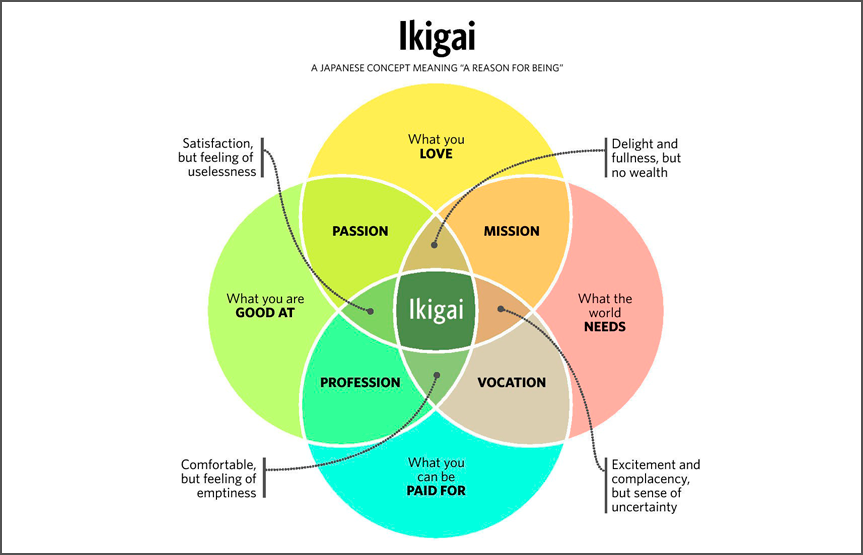
\includegraphics[width=0.8\textwidth]{img/ikigai.png} \\
    \tiny{\url{https://zekluu.com/en/self-development-ikigai-el-sentido-de-la-vida/}}
  \end{figure}
\end{frame}

\begin{frame}{}
  \centering
  \pause
  \textit{Winners forget they're in a race, they just love to run.} \\
  \vspace{3mm}
  \hfill \textit{Simon Wilder (With Honors, 1994)} \\
\end{frame}

\begin{frame}{Ești la o bere cu \ldots}
  \begin{itemize}
    \pause
    \item Jeff Bezos
    \pause
    \item Barack Obama
    \pause
    \item Arnold Schwarzenegger
  \end{itemize}
  \pause
  Cât de mult contează pentru tine \textbf{ce} au obținut? Cât de mult contează pentru tine \textbf{cum} au obținut?
\end{frame}

\begin{frame}{Călătorie și destinație}
  \begin{enumerate}
    \item ne este indiferentă călătoria, nu avem destinație
    \item ne place călătoria, nu avem destinație
    \item ne este indiferentă călătorie, avem destinație
    \item ne place călătoria, avem destinație
  \end{enumerate}
\end{frame}

\begin{frame}{Destinația / Obiectivele contează pentru că \ldots}
  \begin{itemize}
    \pause
    \item dau direcție
    \pause
    \item focalizează
    \pause
    \item sunt împărtășite de un grup / o comunitate / o organizație
    \pause
    \item sunt ușor de definit, sunt obiective (adjectiv), sunt măsurabile
  \end{itemize}
\end{frame}

\begin{frame}{Destinația / Obiectivele contează, dar \ldots}
  \begin{itemize}
    \pause
    \item sunt reci, seci
    \pause
    \item oferă satisfacție temporară
    \pause
    \item sunt nepersonale, sunt adesea dictate din ,,exterior''
    \pause
    \item sunt tangibile; ce faci după ce ai atins obiectivul?
  \end{itemize}
\end{frame}

\begin{frame}{}
  \centering
  \LARGE
  Fericirea este un proces, nu o finalitate. O călătorie, nu o destinație.
\end{frame}

\begin{frame}{Pe scurt \ldots}
  \centering
  \LARGE
  \pause
  Destinația contează. \\
  \pause
  Călătoria contează. \\
  \pause
  Călătoria $>$ destinația
\end{frame}

\begin{frame}{Destinații vs. călătorii}
  \begin{itemize}
    \pause
    \item vreau să am 1 milion de dolari
    \pause
    \item vreau să construiesc o idee care să fie utilă, să ajute lumea
  \end{itemize}
  \begin{itemize}
    \pause
    \item vreau să fiu profesor rang I / whatever
    \pause
    \item vreau să inspir / cresc copiii / studenții, să ajungă oameni buni
  \end{itemize}
  \begin{itemize}
    \pause
    \item vreau să fiu primar / președinte
    \pause
    \item vreau să îmbunătățesc lucrurile în orașul / județul / țara mea
  \end{itemize}
\end{frame}

\begin{frame}{Întrebări grele}
  \onslide<2->{Care este sensul vieții? De ce trăim?\\}
  \onslide<4->{evoluție, creștere, delta\\}
  \vspace{1cm}
  \onslide<3->{Ce ne motivează?\\}
  \onslide<5->{autonomy, mastery, purpose\\}
\end{frame}

\begin{frame}{Evoluție}
  \centering
  \pause
  comparație cu tine ieri \\
  \pause
  creștere, senzația că ești mai bun \\
  \pause
  ești mai util ție și celorlați (dăm spre purpose)
\end{frame}

\begin{frame}{Mastery}
  \url{https://twitter.com/SeekMastery/}
  \begin{itemize}
    \item desire
    \item consistency
    \item passion
  \end{itemize}
\end{frame}

\begin{frame}{Purpose}
  \centering
  \pause
  ceva mai mult decât tine \\
  \pause
  un țel constant, nu ceva tangibil \\
  \pause
  parte constantă a călătoriei \\
  \pause
  ultimate level: life mission
\end{frame}

\begin{frame}{Cum ajung la \ldots}
  \centering
  \pause
  evoluție, creștere \\
  \pause
  mastery \\
  \pause
  purpose \\
  \pause
  călătorie cu plăcere \\
  \pause
  fericire constantă (ca proces) \\
  \pause
  {\large\textbf{Nu există rețete, dar ...}}
\end{frame}

\begin{frame}{Întrebări pe care să ți le pui}
  \centering
  \large
  \pause
  Ce-mi place / ce mă împinge înainte cu adevărat? (e de săpat în tine) \\
  \vspace{1cm}
  \pause
  Presupunând că aș avea totul, ce m-ar face să mă trezesc în fiecare zi? \\
  \vspace{1cm}
  \pause
  Ce versiune a lumii m-ar afecta cel mai mult? (ți-ai pierde drive-ul de a te trezi în fiecare zi) \\
\end{frame}

\begin{frame}{Clișeu de final}
  \centering
  \pause
  \textit{The journey of a thousand miles begins with one step.} \\
  \vspace{3mm}
  \hfill \textit{Lao Tzu} \\
\end{frame}

\begin{frame}{Resurse}
  \begin{itemize}
    \item slide-urile prezentării: \url{https://www.slideshare.net/razvandeaconescu/}
    \item cod sursă prezentare: \url{https://github.com/razvand/slides}
    \item \url{https://twitter.com/ProfFeynman}
    \item Seth Godin \url{https://seths.blog/}
    \item Daniel Pink: Drive (2009)
    \item Scott Adams: How to Fail at Almost Everything and Still Win Big: Kind of the Story of My Life (2013)
    \item \url{https://www.scottadamssays.com/2013/11/18/goals-vs-systems/}
  \end{itemize}
\end{frame}

\end{document}
